\Chapter{Tesztelés és Eredmények}

A program funkciói a fejlesztés során folyamatosan tesztelésre kerültek, alapvetően manuálisan. Az algoritmus, illetve a szemantikus verziózás tesztelése végül a statisztikai vizsgálat során automatikusan is megtörtént, bár nem ez volt annak a résznek a célja. Ennek következtében derült ki az algoritmusnál is tárgyalt hiba, miszerint nem számított bizonyos átlagtól eltérő esetekre, amely a ciklus végtelen futását eredményezte.\\

Ebben a szekcióban a program felhasználása, illetve a használatával szerzett eredmények elemzése kerül ismertetésre.

\section{Használat}

\begin{figure}[!h]
	\centering
	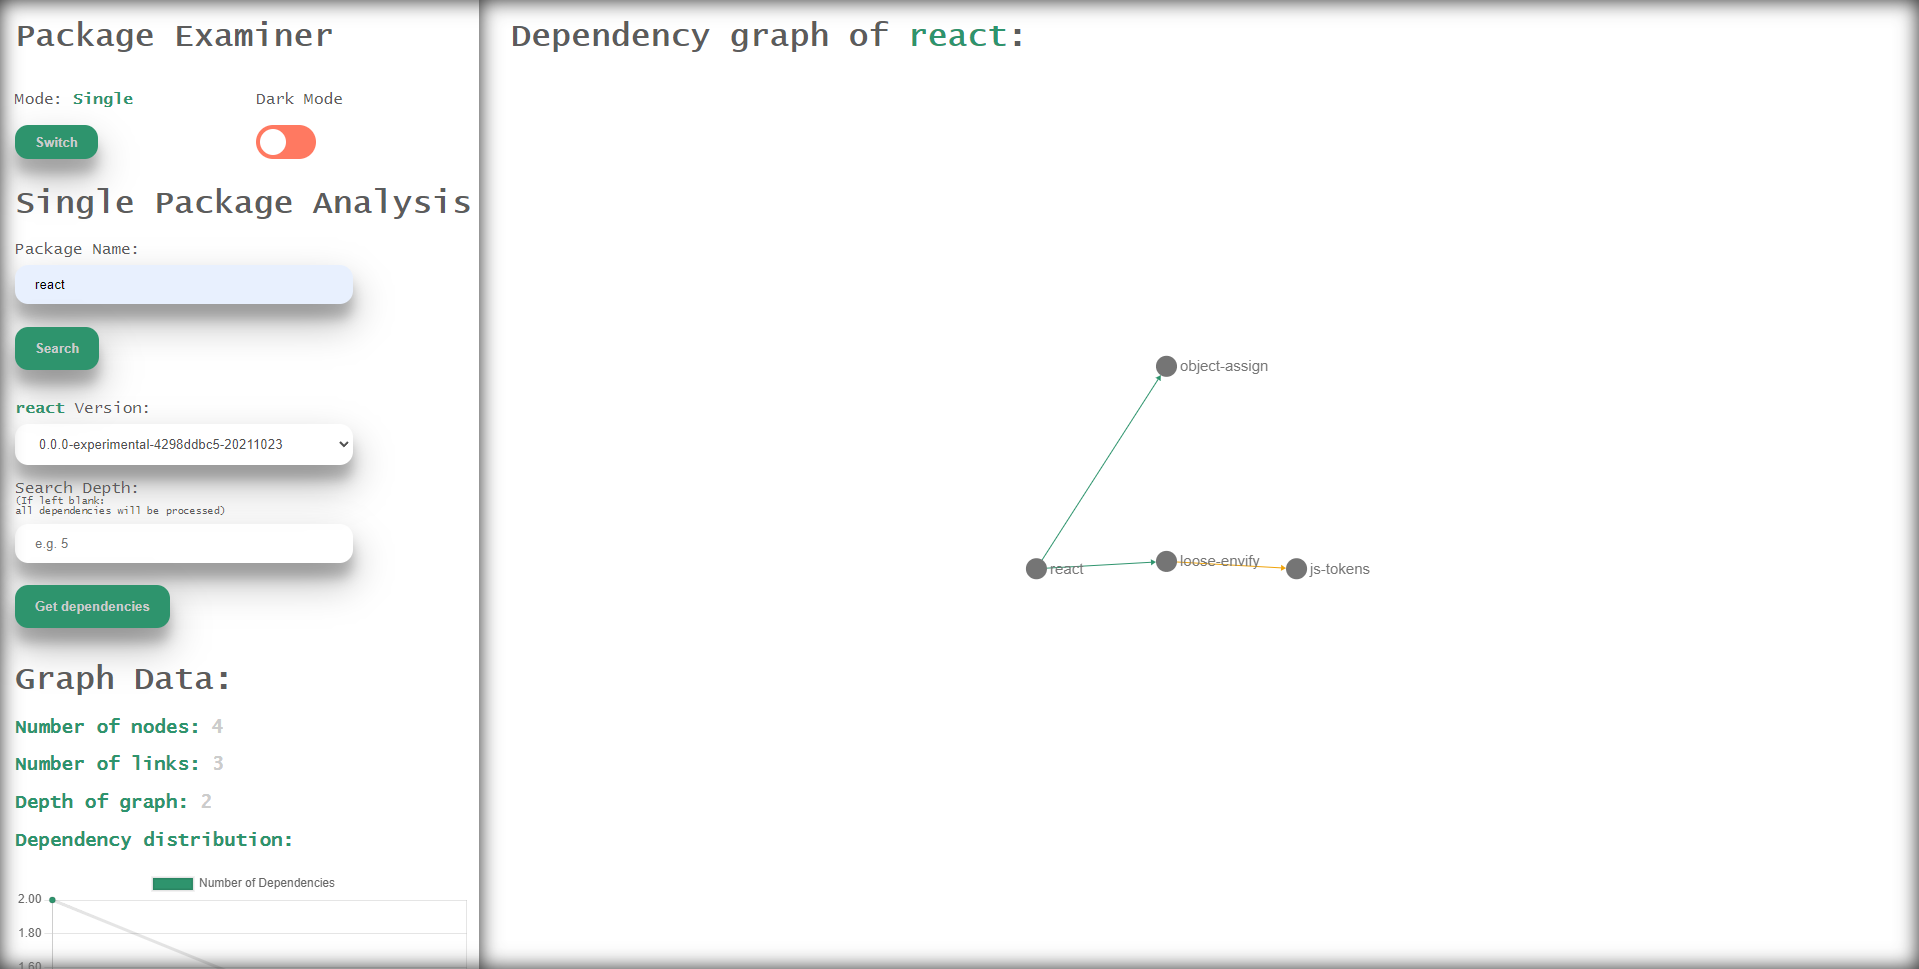
\includegraphics[scale=0.2]{images/examiner.png}
	\caption{Egy Csomagos Mód}
	\label{fig:examiner}
\end{figure}

\begin{itemize}
	\item Első lépésként meg kell adni a csomag nevét és keresni a (Search) gombbal.
	\item Helyes csomagnév esetén feltöltődik a verziók listája, innen tetszőlegesen kell választani egyet.
	\item Opcionálisan megadható, hogy keresés mennyire legyen mély
	\item Végül a (Get dependencies) gomb megnyomásával lehet elindítani a folyamatot.
	\item Az elkészült ábra görgővel és egérgomb lenyomva tartásával interaktívan mozgatható, nagyítható. A Sidebar pedig lefelé görgethető a gráfelemzés információinak megtekintéséhez.
\end{itemize}

\pagebreak

\textbf{A két mód közötti váltást a (Switch) gomb segítségével lehet megtenni.}

\begin{figure}[!h]
	\centering
	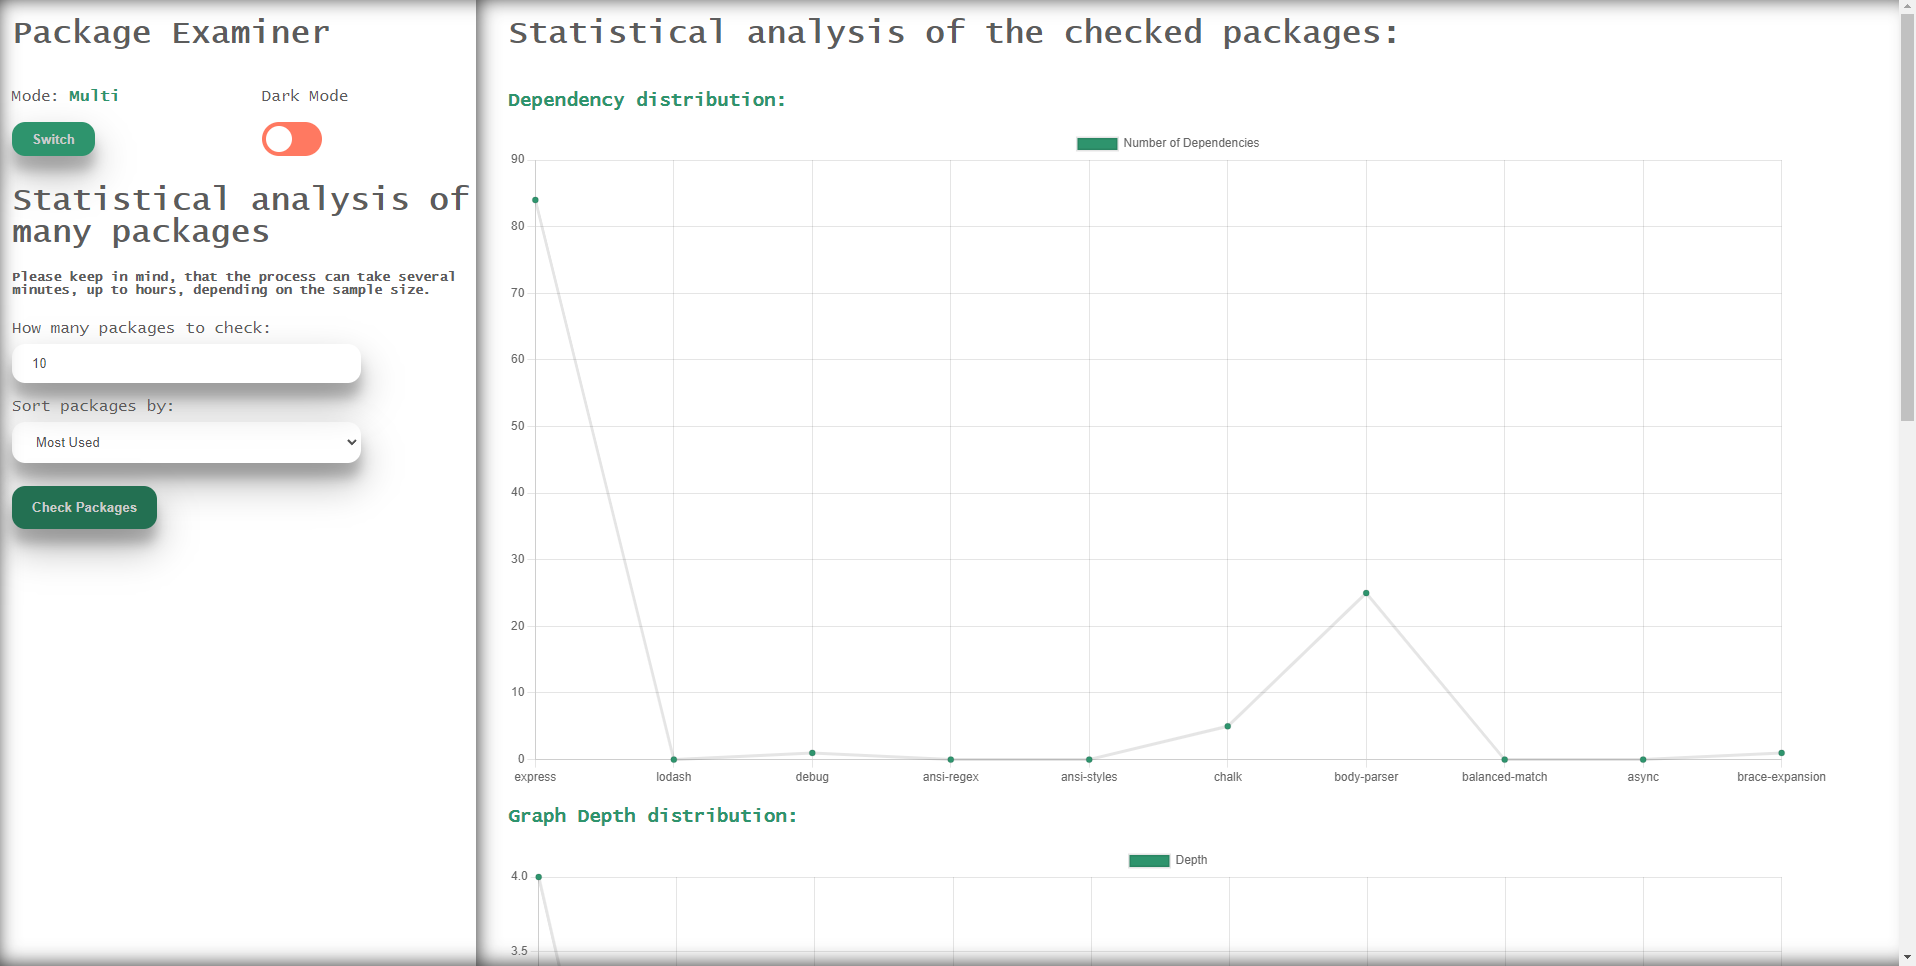
\includegraphics[scale=0.2]{images/statistics.png}
	\caption{Több Csomagos Mód}
	\label{fig:examiner}
\end{figure}

\begin{itemize}
	\item Először a vizsgált csomagok mennyiségét szükséges megadni.
	\item A lefelé gördülő listából pedig a sorrendbe állítási elvet kell kiválasztani, alapértelmezett a leggyakrabban használt csomagok elve.
	\item A folyamatot a (Check Packages) gombra kattintással lehet elindítani.
\end{itemize}

\section{Eredmények}

A korábban tárgyalt mérete és csomagmennyisége miatt az npm Registry egészét túl hosszas és költségigényes lenne elemezni, így az első ezer leggyakrabban használt csomagról, mint "reprezentatívan leszűkített Registryről" készült statisztikai elemzés, amely a következő eredményeket adta, a függőségek száma szerint csökkenő sorrendben rendezve a csomagadatokat:

\begin{figure}[!h]
	\centering
	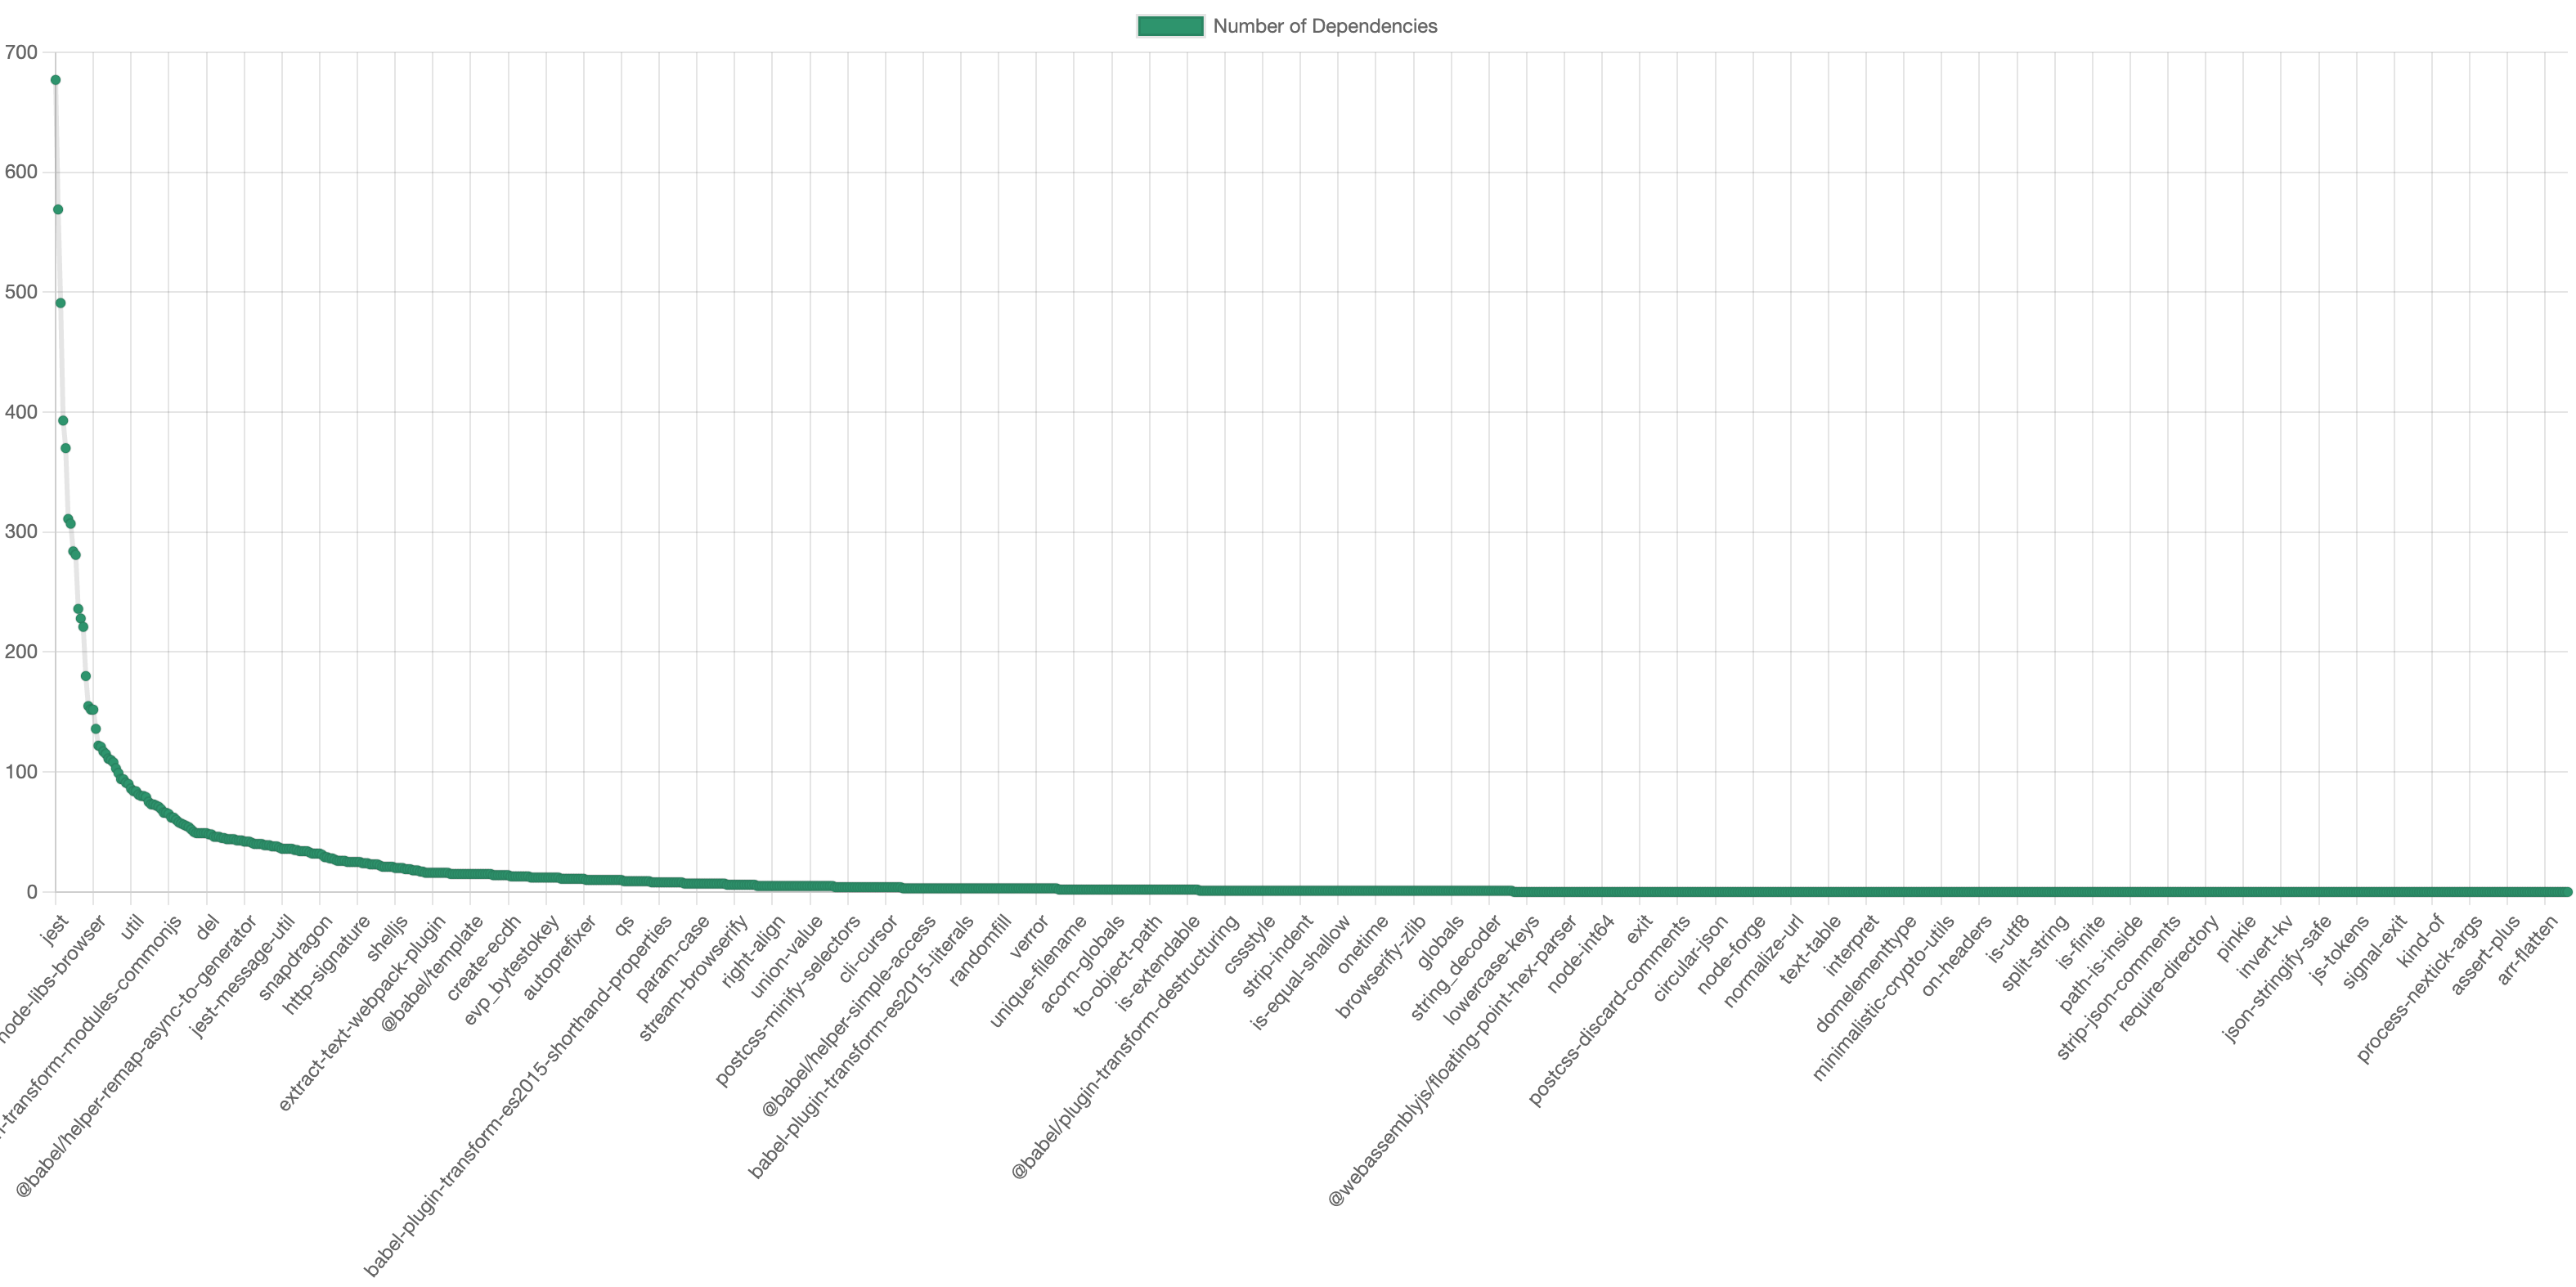
\includegraphics[scale=0.12]{images/depdist.png}
	\caption{Függőségek számának eloszlása}
	\label{fig:depdist}
\end{figure}  

\begin{figure}[!h]
	\centering
	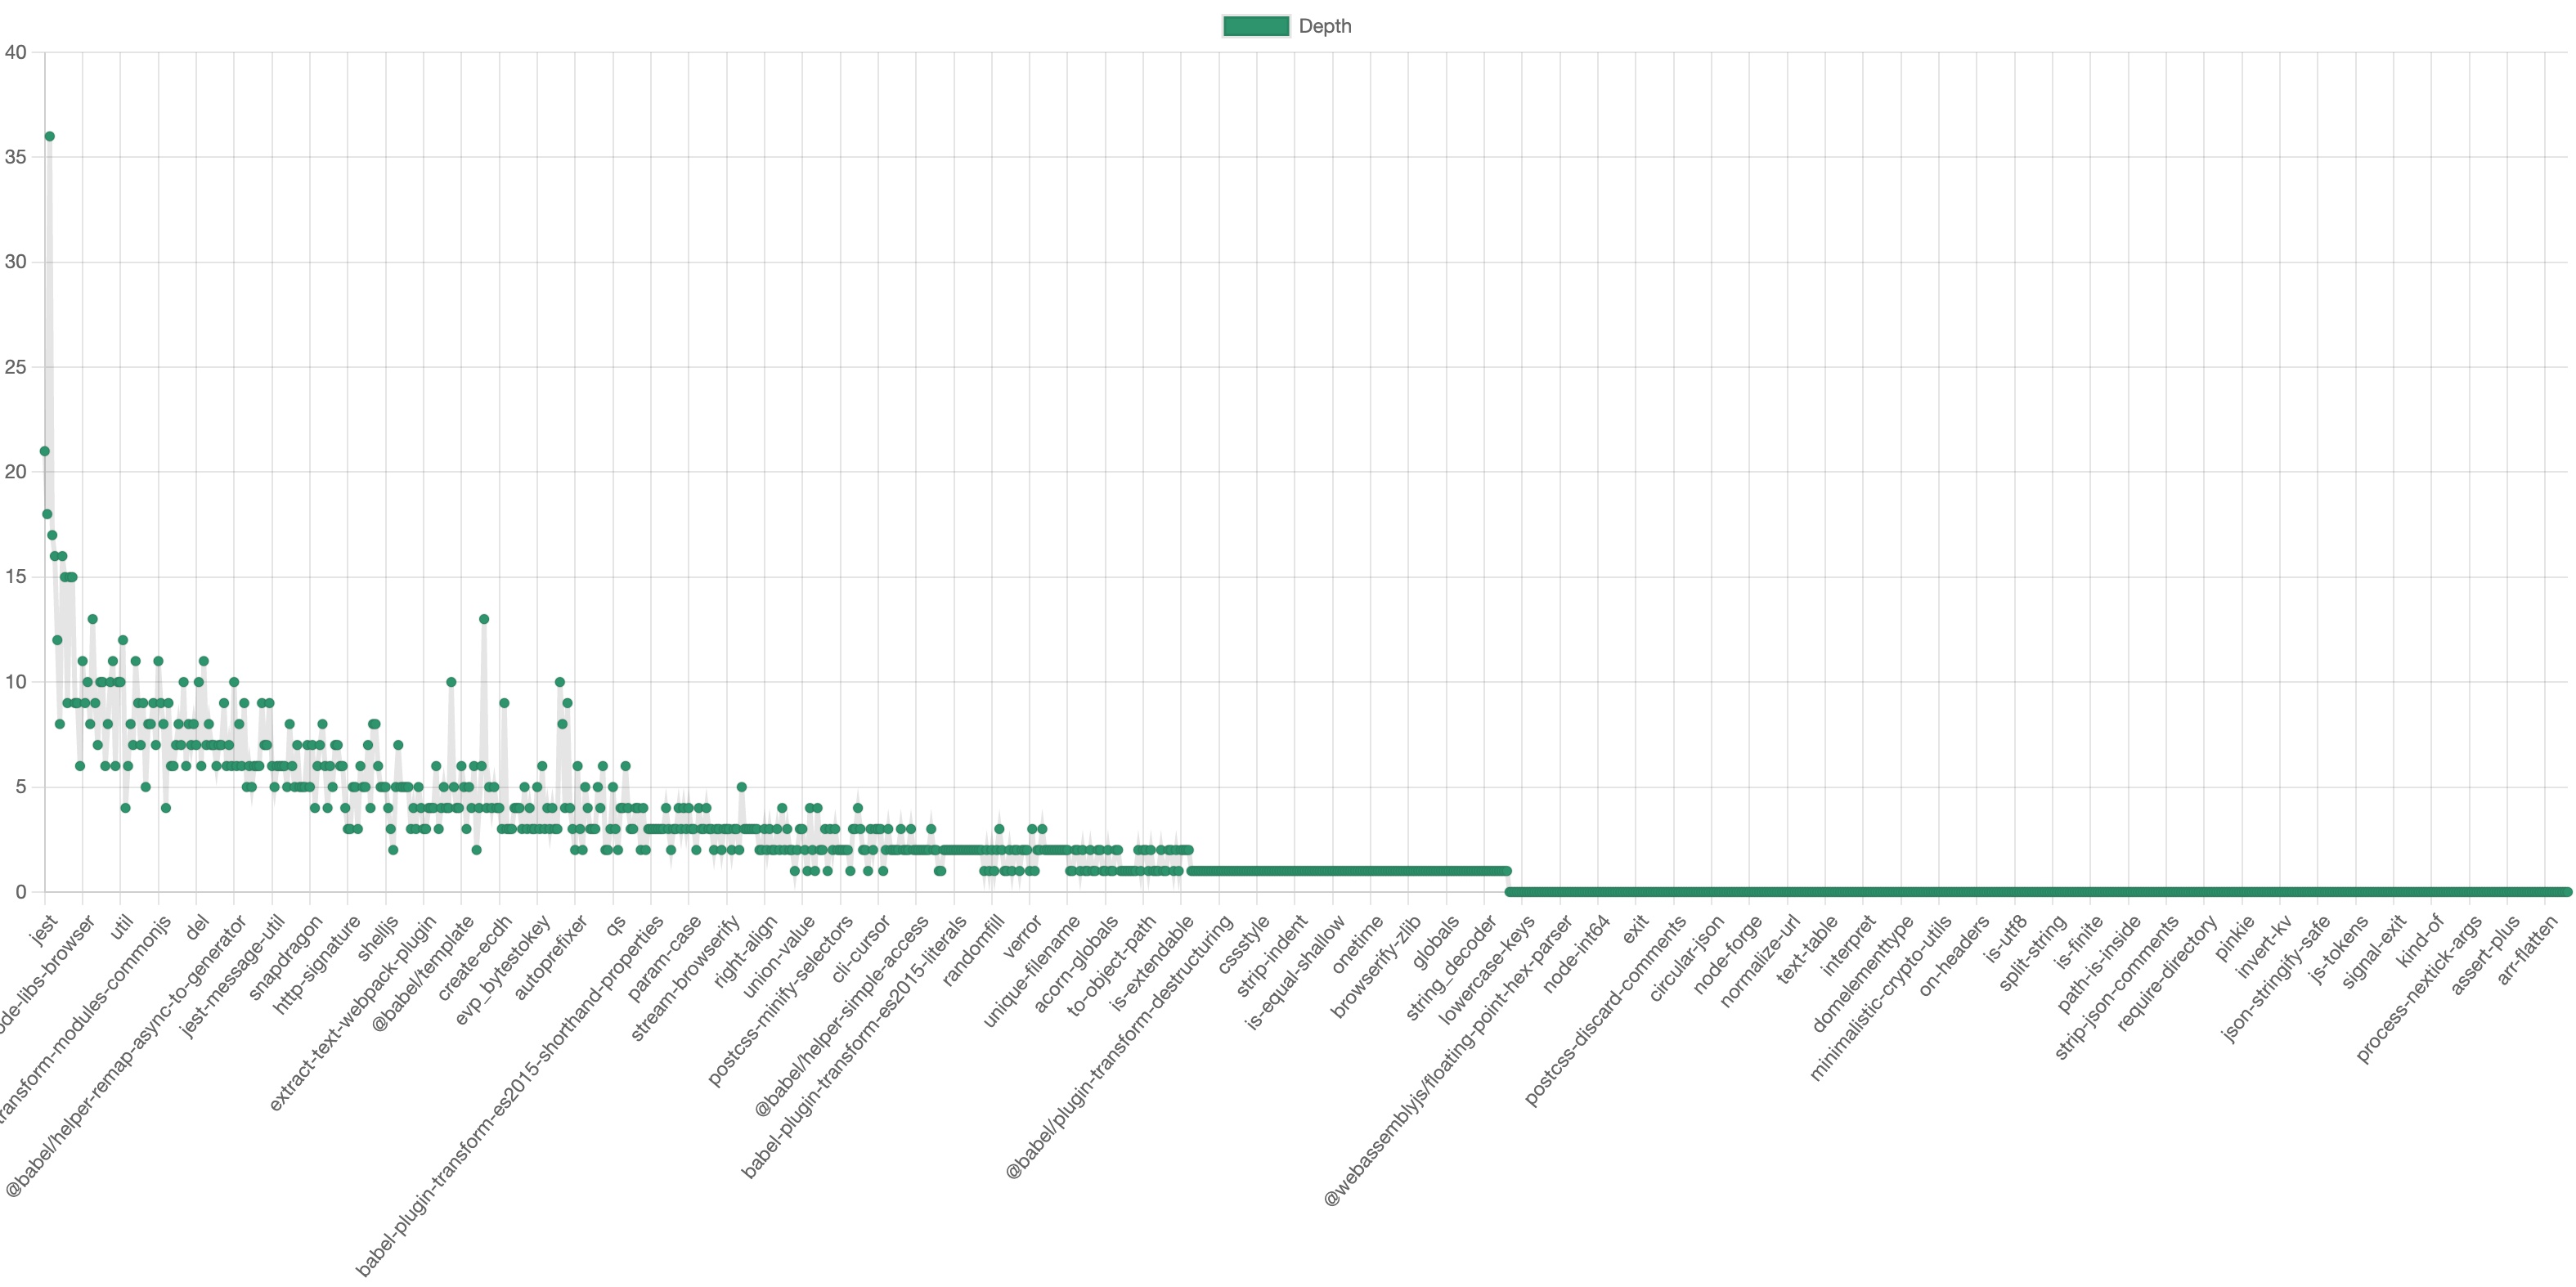
\includegraphics[scale=0.12]{images/graphdepth.png}
	\caption{Csomagonkénti gráfmélység}
	\label{fig:graphdepth}
\end{figure}

\begin{figure}[!h]
	\centering
	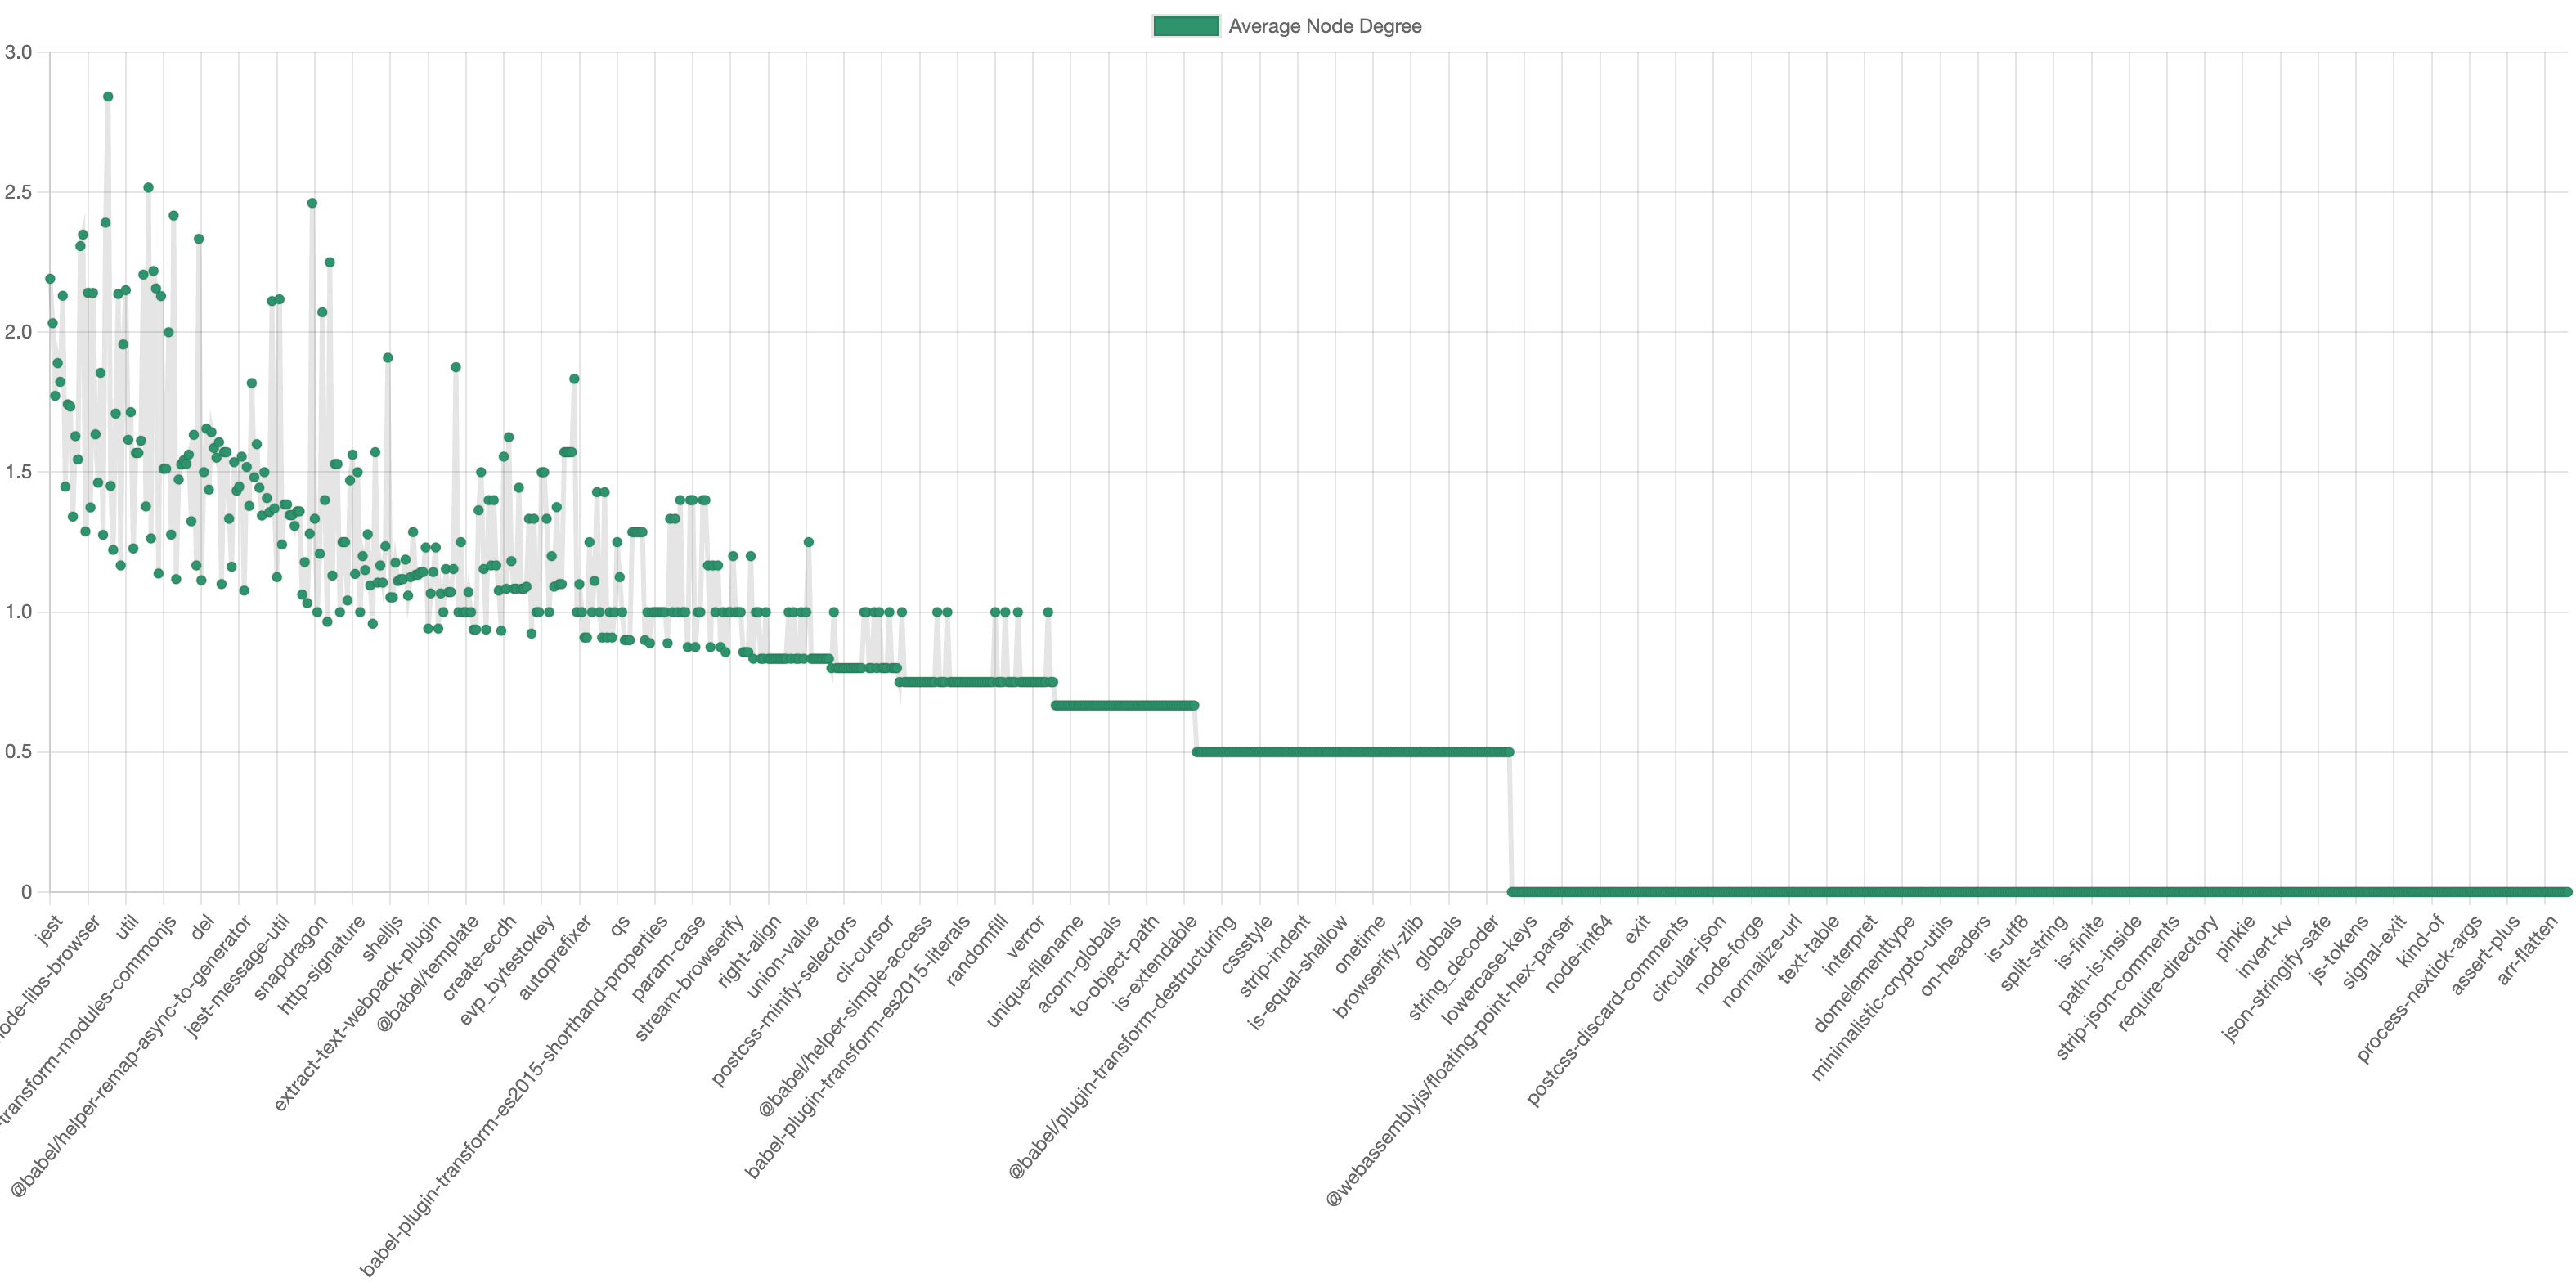
\includegraphics[scale=0.12]{images/avgdegree.png}
	\caption{Csomagonkénti átlagos fokszám}
	\label{fig:avgdegree}
\end{figure}

\begin{figure}[!h]
	\centering
	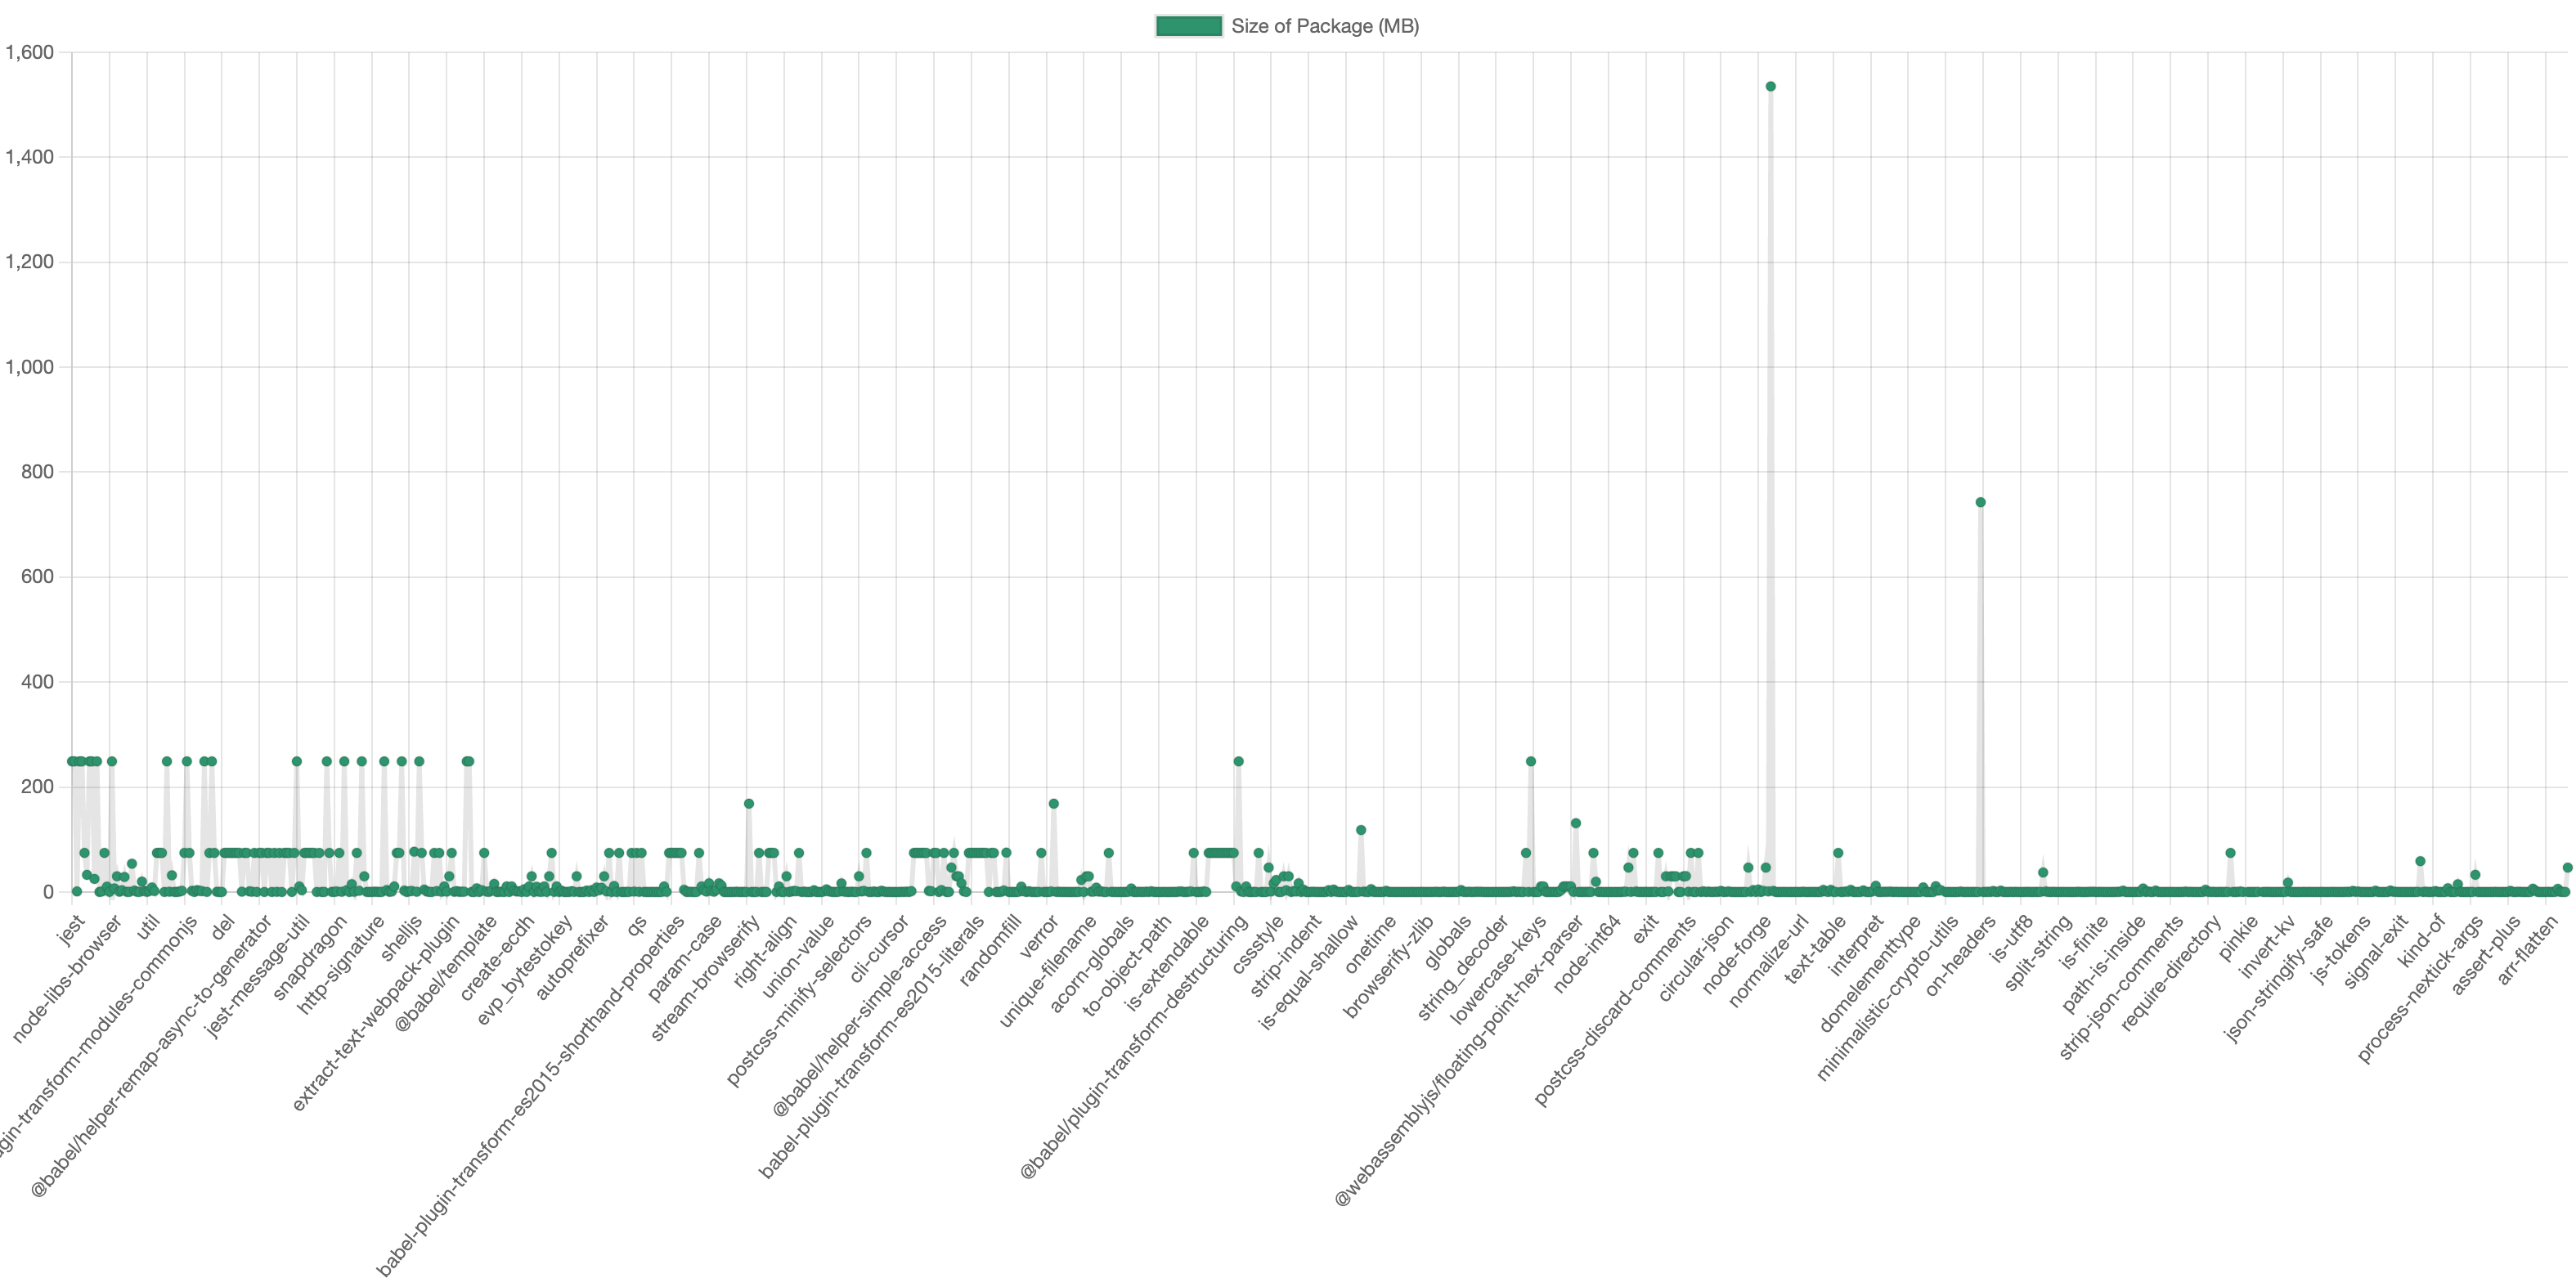
\includegraphics[scale=0.12]{images/pkgsize.png}
	\caption{Csomagméret(MB-ban megadott) eloszlás}
	\label{fig:pkgsize}
\end{figure}

\begin{figure}[!h]
	\centering
	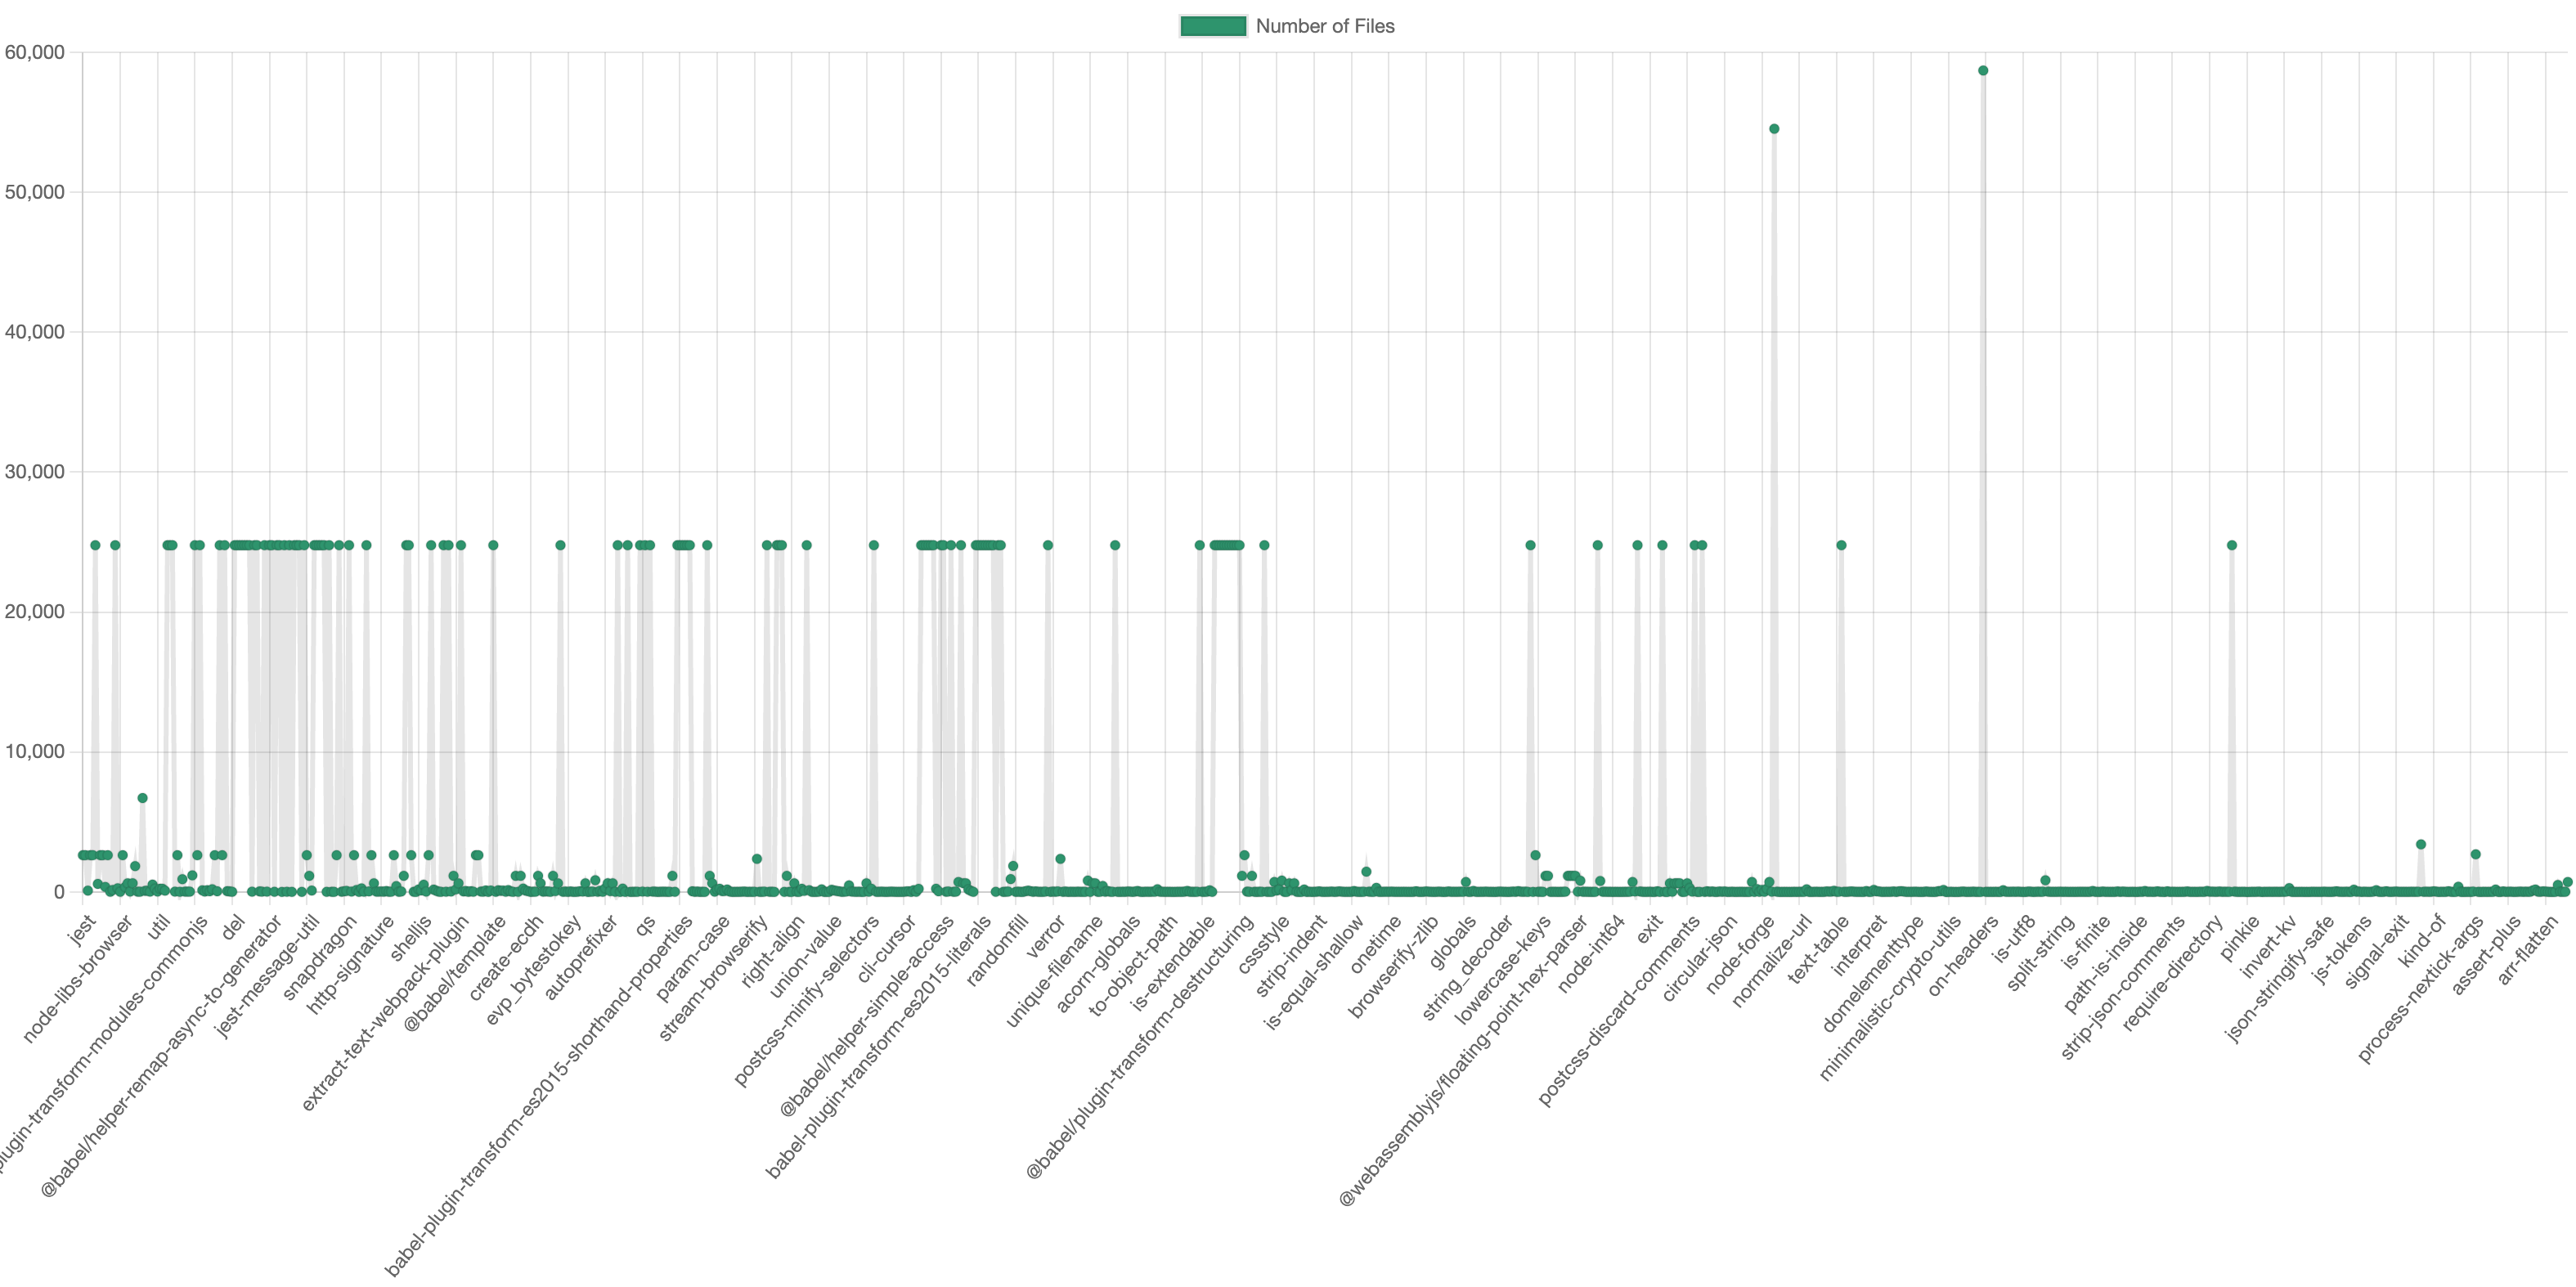
\includegraphics[scale=0.12]{images/numoffiles.png}
	\caption{Csomagonkénti fájlok száma}
	\label{fig:numoffiles}
\end{figure}

\begin{figure}[!h]
	\centering
	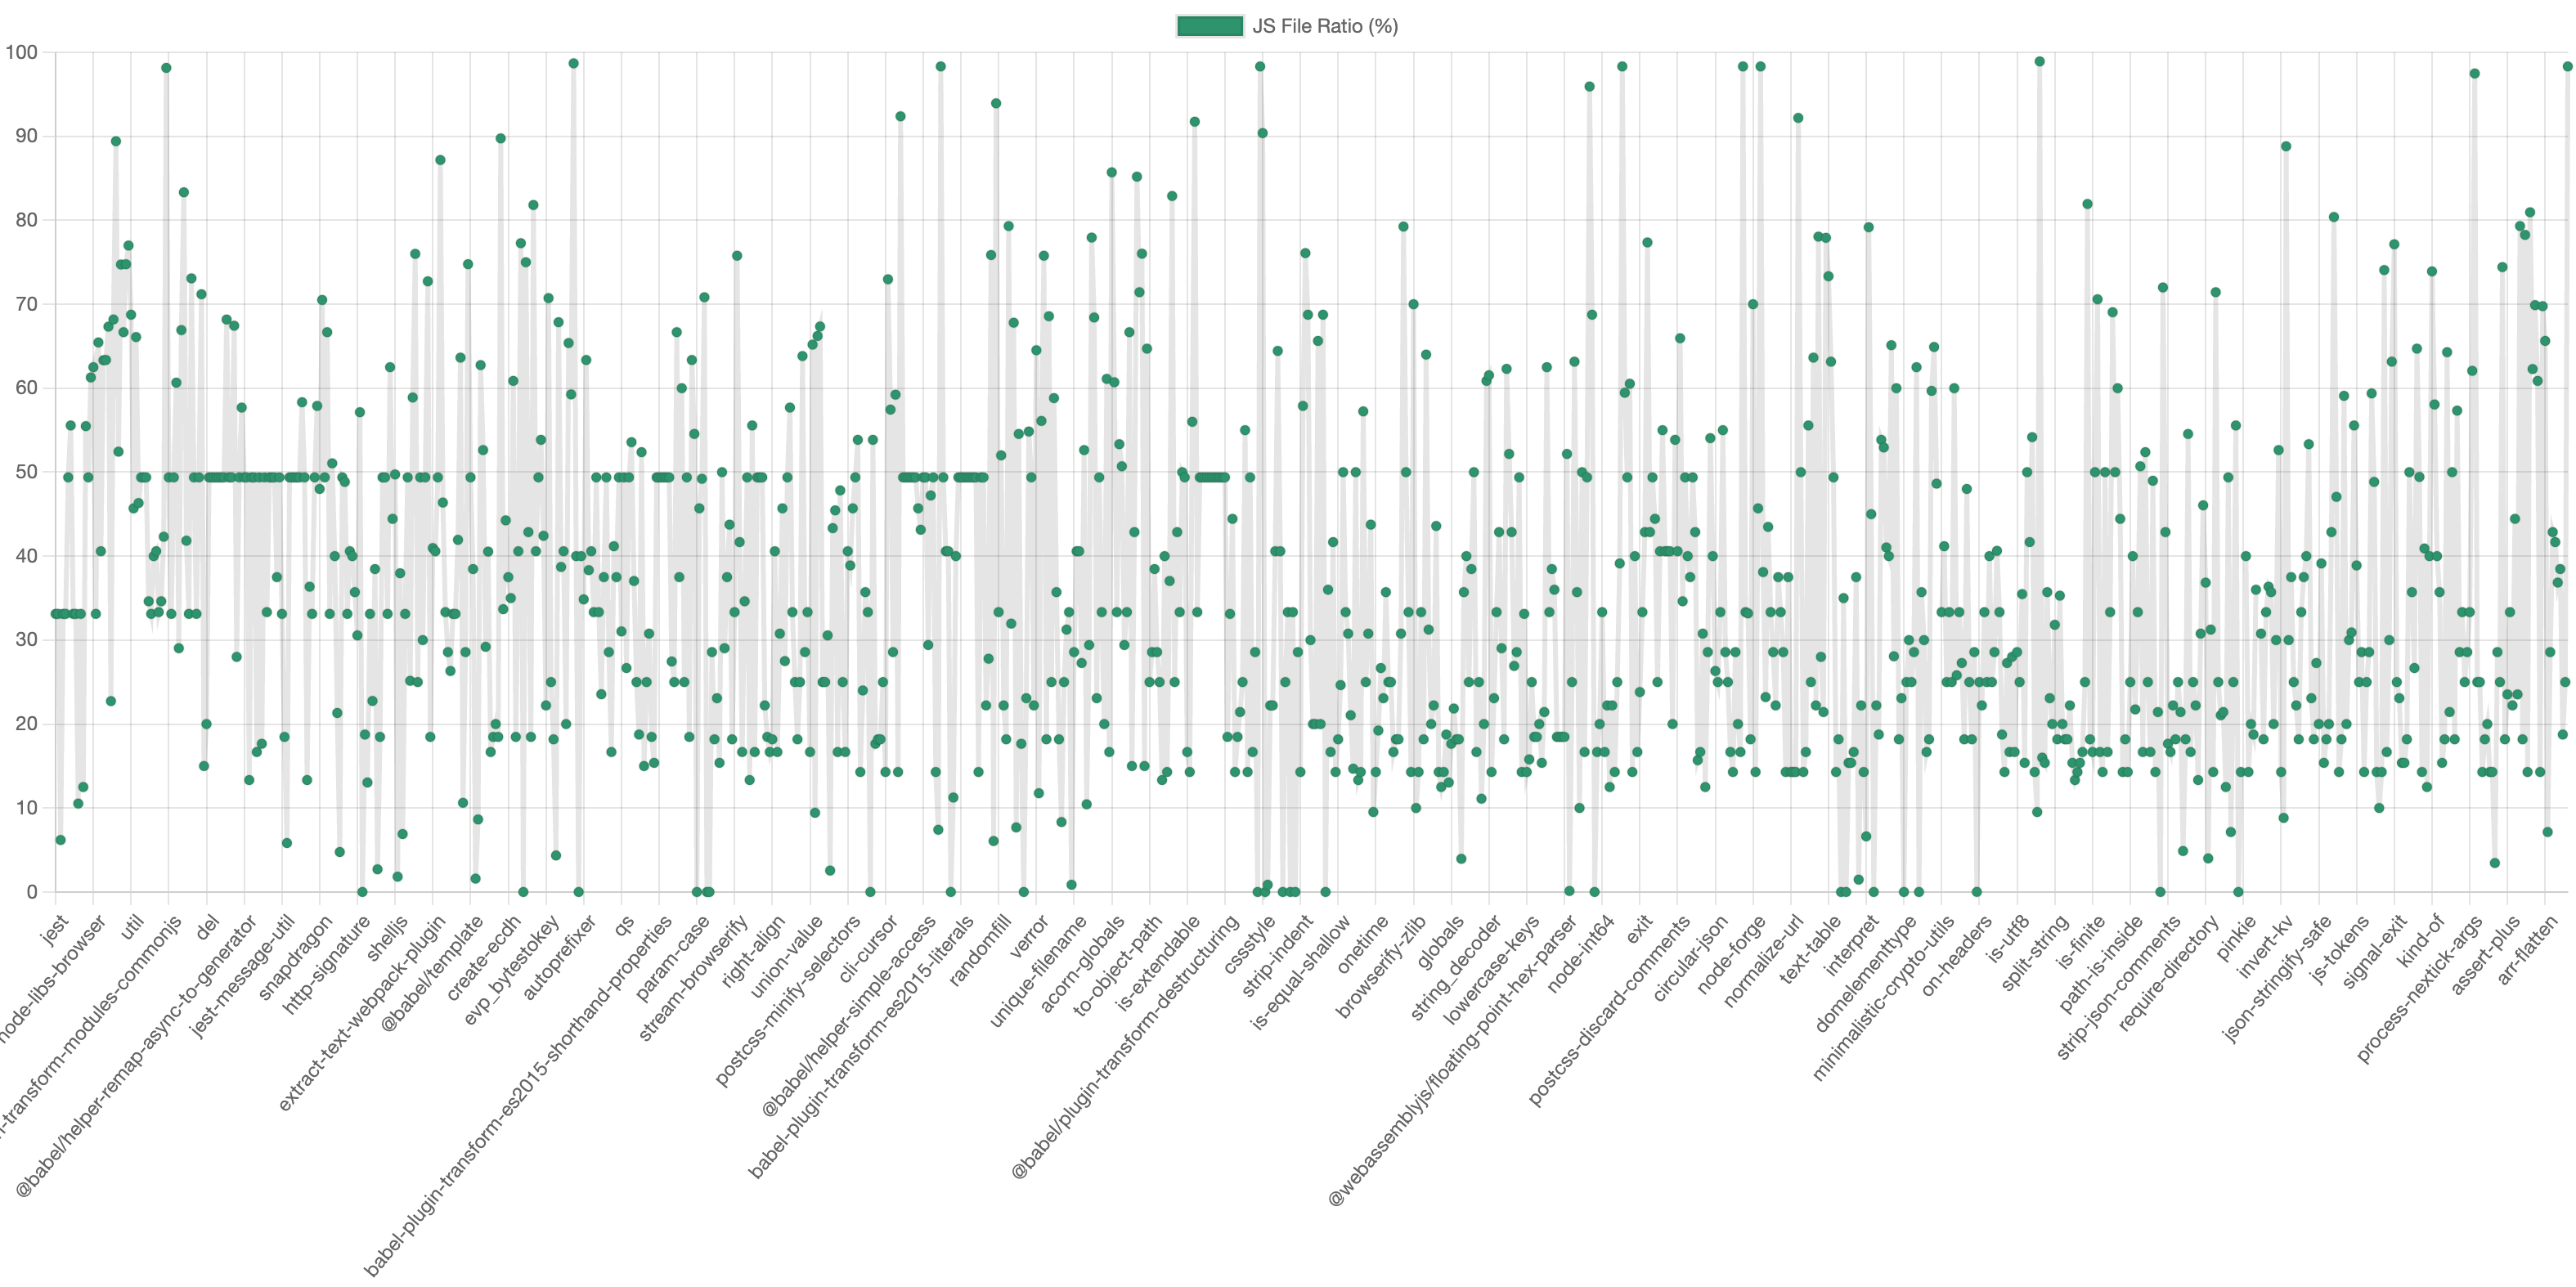
\includegraphics[scale=0.12]{images/jsratio.png}
	\caption{Csomagonkénti JavaScript fájlok aránya (\%)}
	\label{fig:jsratio}
\end{figure}

\begin{figure}[!h]
	\centering
	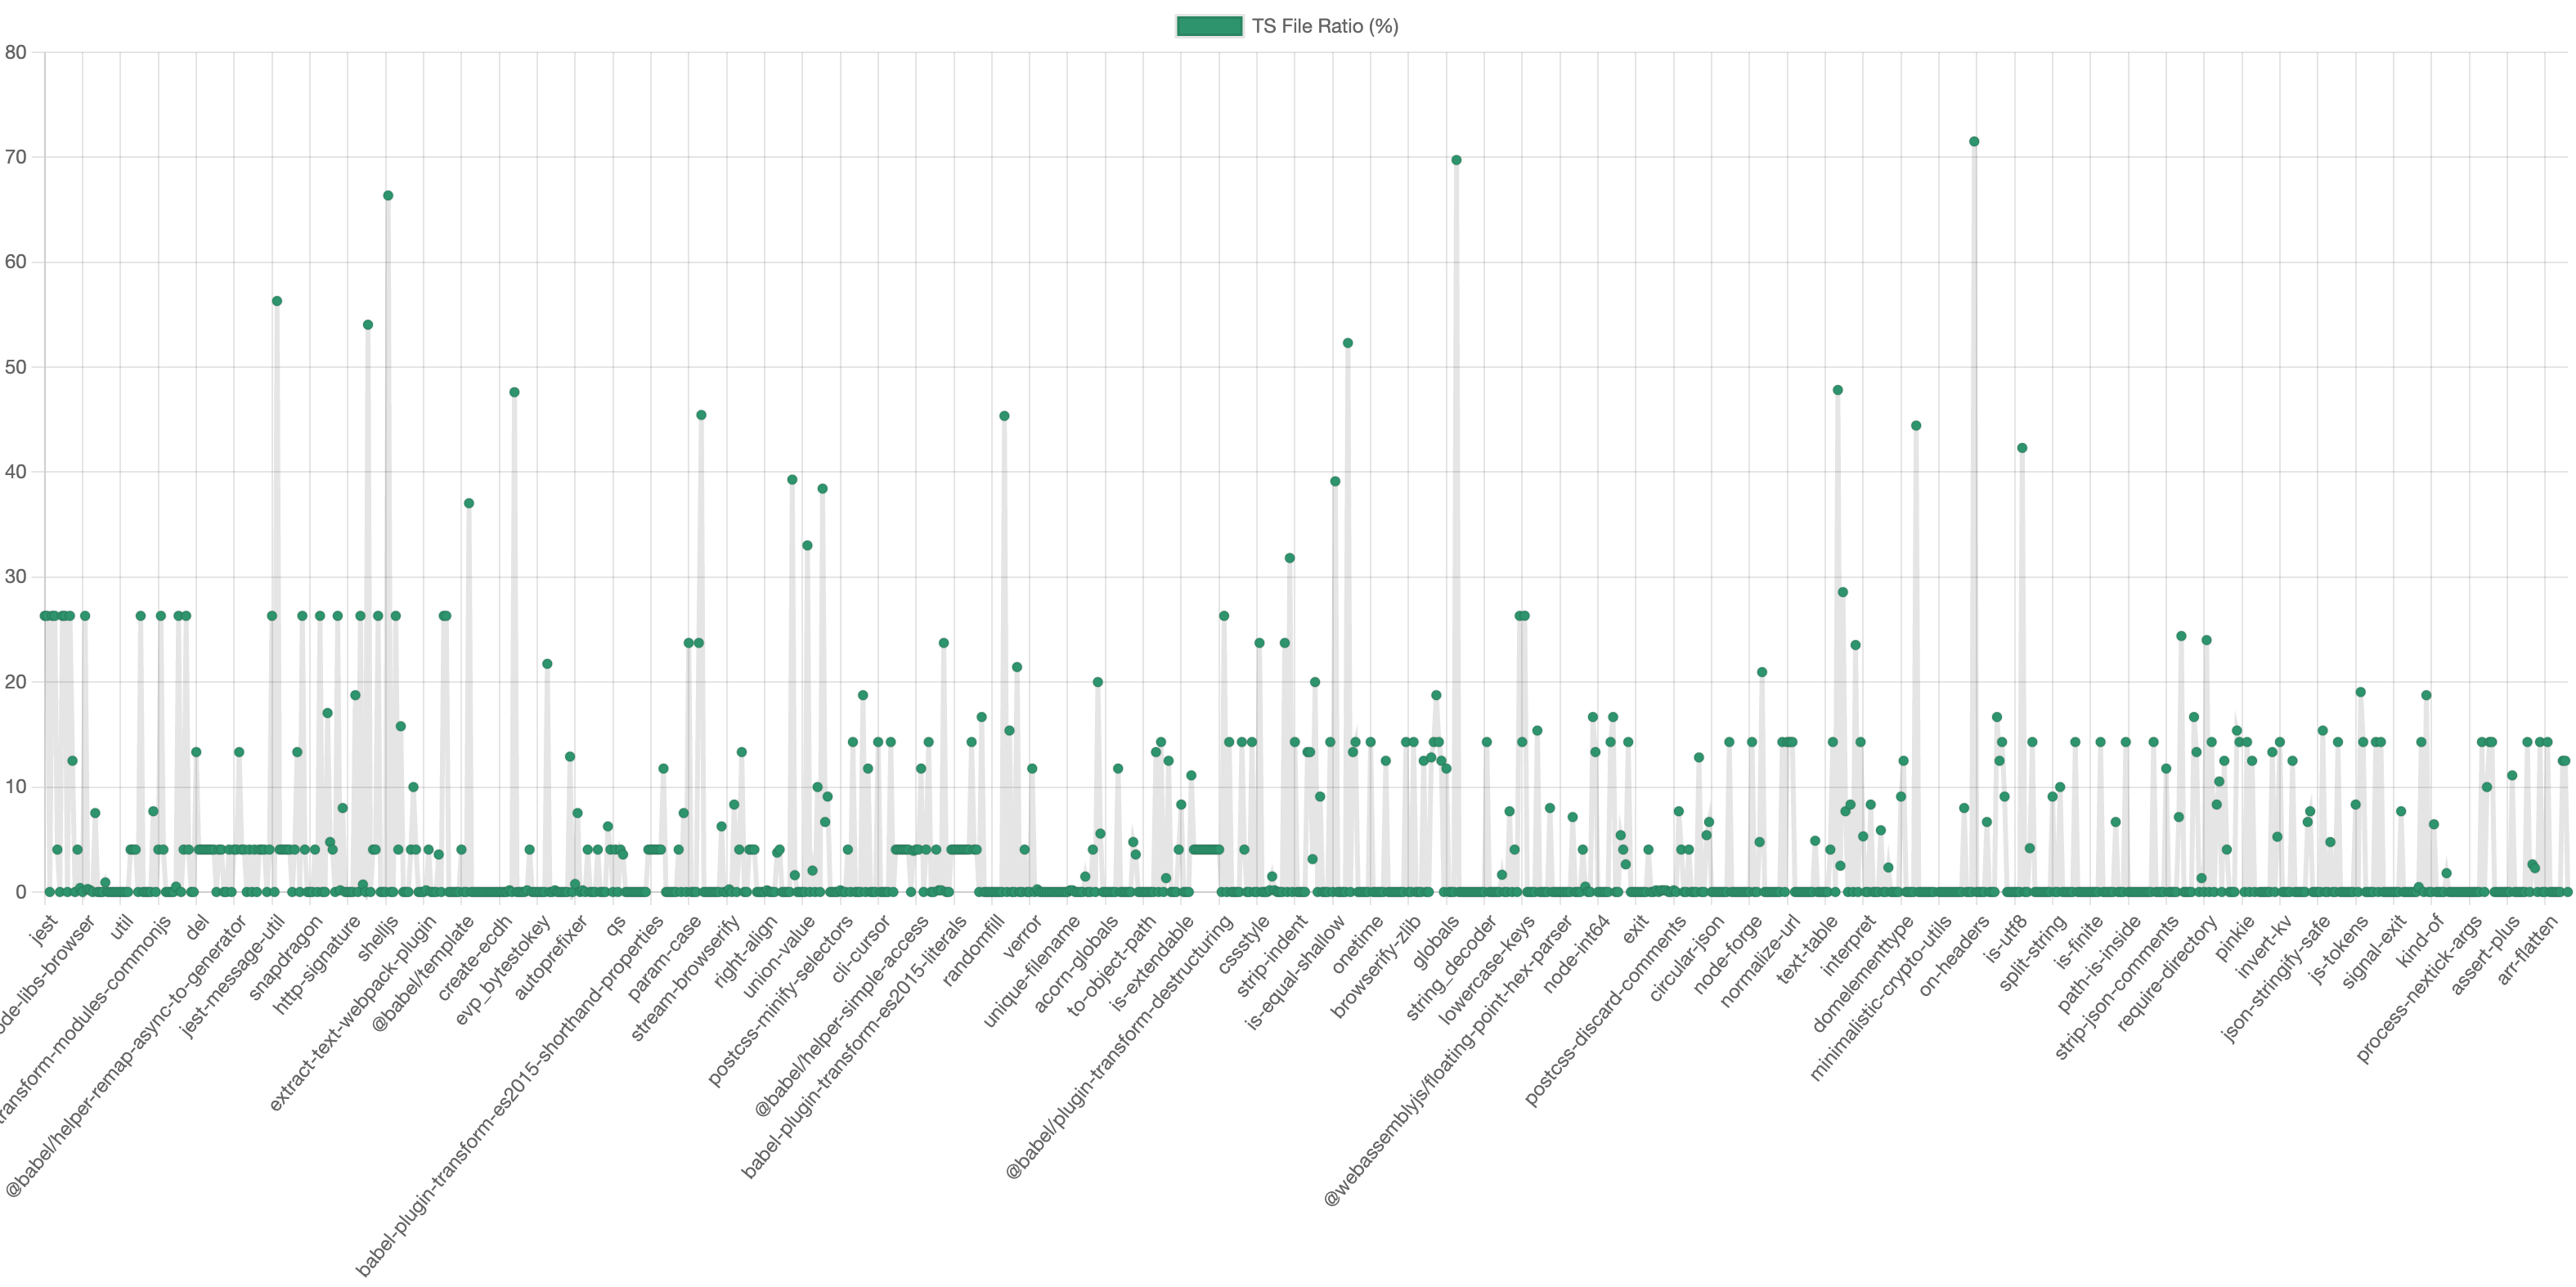
\includegraphics[scale=0.12]{images/tsratio.png}
	\caption{Csomagonkénti TypeScript fájlok aránya (\%)}
	\label{fig:tsratio}
\end{figure}

\begin{figure}[!h]
	\centering
	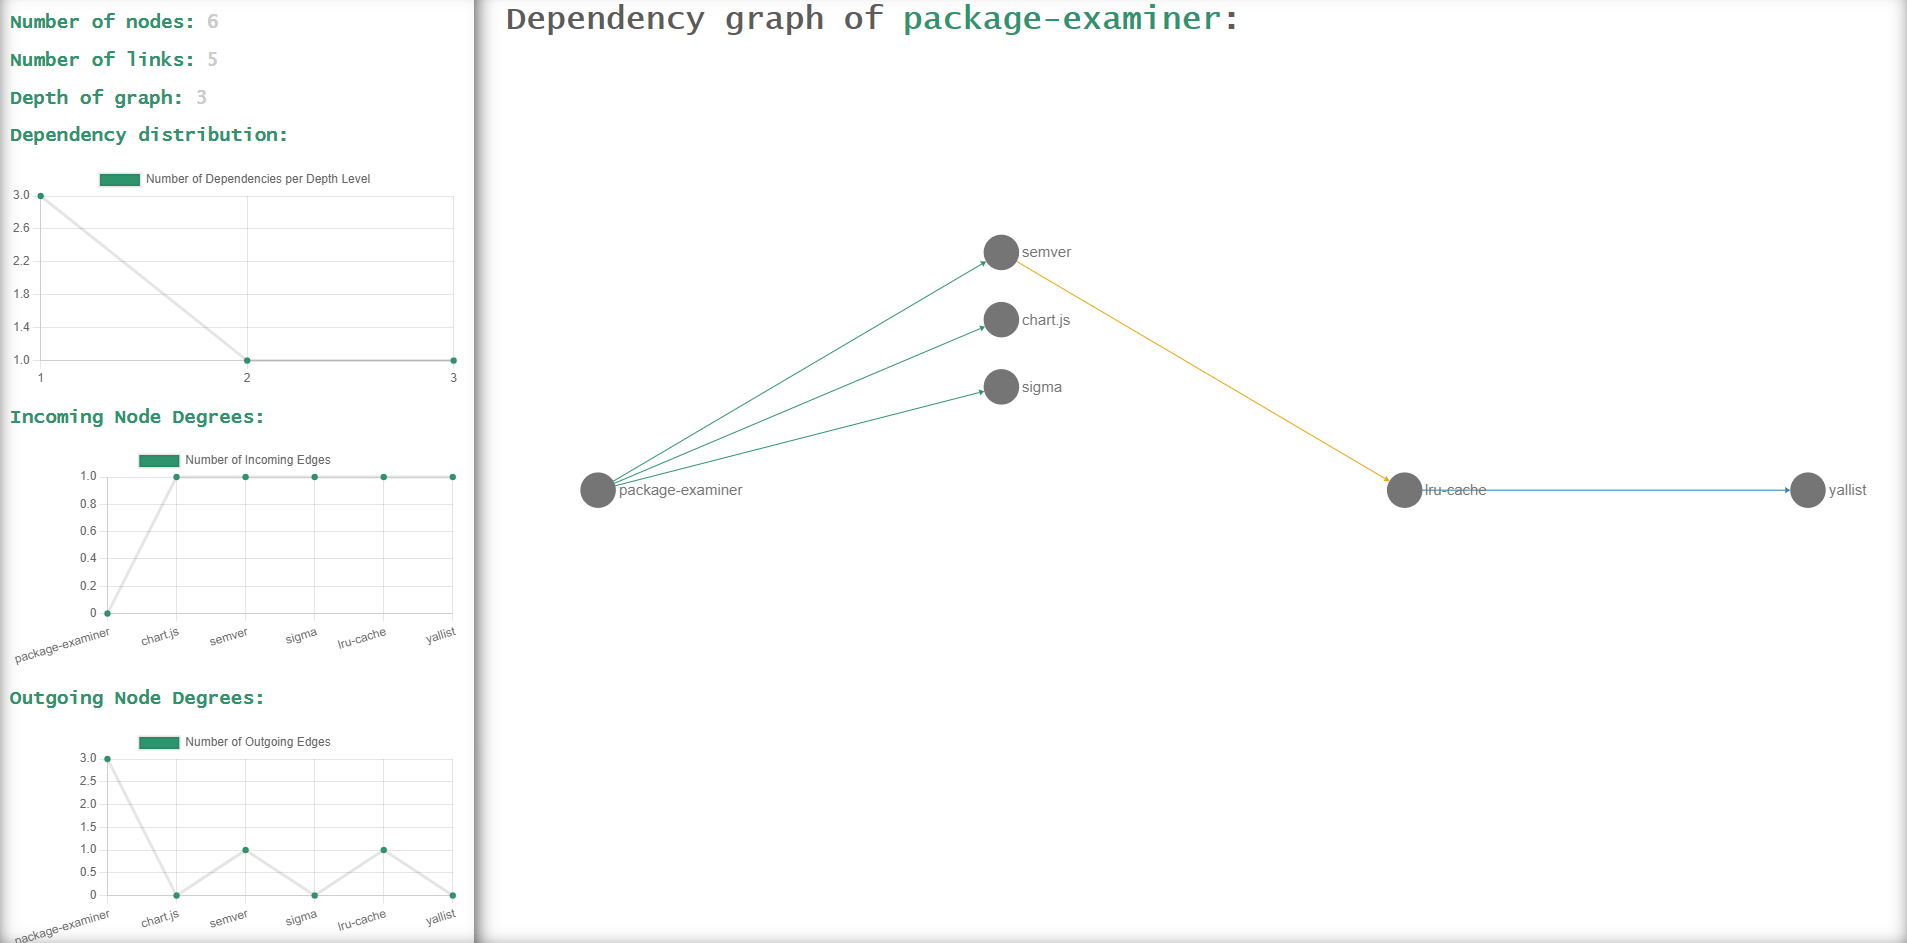
\includegraphics[scale=0.3]{images/package-examiner.png}
	\caption{A Package Examiner függőségeinek elemzése}
	\label{fig:package-examiner}
\end{figure}